% Presentation structure
%
% Part I: Preliminaries
%   The @Web platform
%   @Web ontology
%   Annotated tables
%   Guidelines
%   Examples constraints
%
% Part II: RDF data validation: survey of the state of the art
%   Shape Expressions
%   SHACL
%   Plain SPARQL
%
% Part III: Implementation
%   Examples of real constraints
%   Live demo
%
% Part IV: Conclusions
%   Conclusions
%   Future work
%   Thanks


\documentclass{beamer}
\usepackage[utf8]{inputenc}
\usepackage{graphicx}
\usepackage{xspace}

% Convenience macros
\newcommand{\atweb}{\textbf{@Web}\xspace}
\newcommand{\partslide}[2]{
  \begin{center}
    \LARGE{#1} \\
    \vspace{0.5cm}
    \huge{#2}
  \end{center}
}

% Remove navigation controls
\usenavigationsymbolstemplate{}

% Slide numbering
\setbeamertemplate{footline}[frame number]

\title{Using SPARQL queries to express integrity constraints in RDF graphs}
\subtitle{
  \vspace{0.5cm}
  Final internship report
}
\author{
  Leandro Lovisolo
}
\date{February 25, 2016}
\institute{
  INRA SupAgro and INRIA GraphiK \\
  Montpellier, France
}

\begin{document}

\begin{frame}
  \titlepage
\end{frame}

%%%%%%%%%%%%%%%%%%%%%%%%%%%%%%%%%%%%%%%%%%%%%%%%%%%%%%%%%%%%%%%%%%%%%%%%%%%%%%%%
% Part I: Preliminaries                                                        %
%%%%%%%%%%%%%%%%%%%%%%%%%%%%%%%%%%%%%%%%%%%%%%%%%%%%%%%%%%%%%%%%%%%%%%%%%%%%%%%%

\begin{frame}
  \partslide{Part I}{Preliminaries}
\end{frame}

\begin{frame}
  \frametitle{Problem statement}

  \begin{itemize}
    \item We have an RDF graph where we store experimental data extracted from
      tables in scientific publications.

    \item The data extraction process is done semi-manually, thus it's very
      error-prone.

    \item Therefore, \textbf{we want to verify the integrity of the annotated
      data automatically.}
  \end{itemize}
\end{frame}

\begin{frame}
  \frametitle{The \atweb platform}
  \framesubtitle{Introduction}

  \begin{itemize}
    \item A software platform used to annotate tables from scientific
      publications in heterogeneous formats (PDF files, Excel spreadsheets,
      etc.)

    \item Data is stored in an RDF graph following a predefined OWL ontology.

    \item Goal of my internship: add integrity constraint checking capabilities
      to the \atweb platform.
  \end{itemize}
\end{frame}

\begin{frame}
  \frametitle{The \atweb platform}
  \framesubtitle{Screenshot}

  \begin{center}
    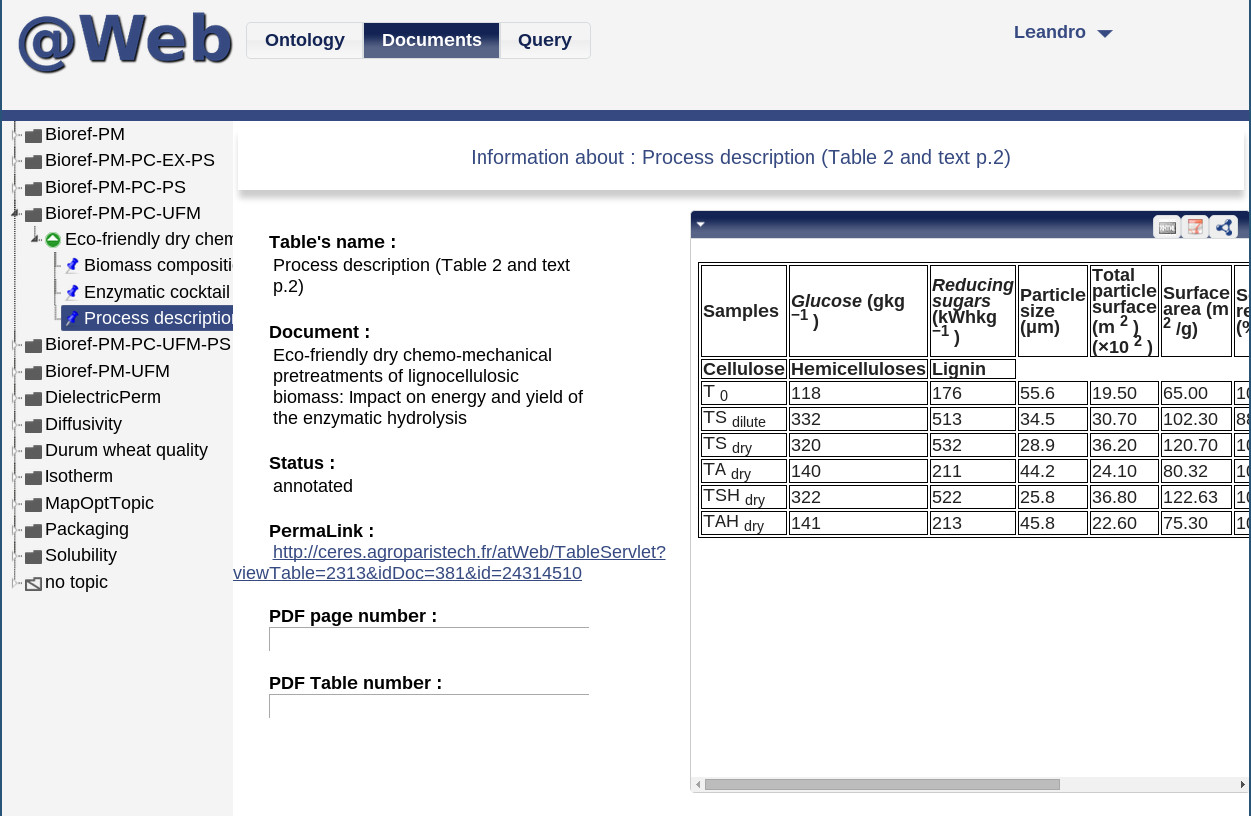
\includegraphics[width=10cm]{atweb-screenshot-document.jpg}
  \end{center}
\end{frame}

\begin{frame}
  \frametitle{The \atweb platform}
  \framesubtitle{$n$-ary relation pattern}

  \begin{itemize}
    \item We're trying to represent experiments composed of many inputs and a
      single output.

    \item An OWL ontology is created where OWL classes are defined for each
      kind of experiment we're interested in representing.

    \item Instances of each experiment class are connected to their respective
      input arguments and output argument via OWL object and data properties.

    \item We're thus defining a pattern for $n$-ary relations.
  \end{itemize}
\end{frame}

\begin{frame}
  \frametitle{The \atweb platform}
  \framesubtitle{Example $n$-ary relation}

  \begin{center}
    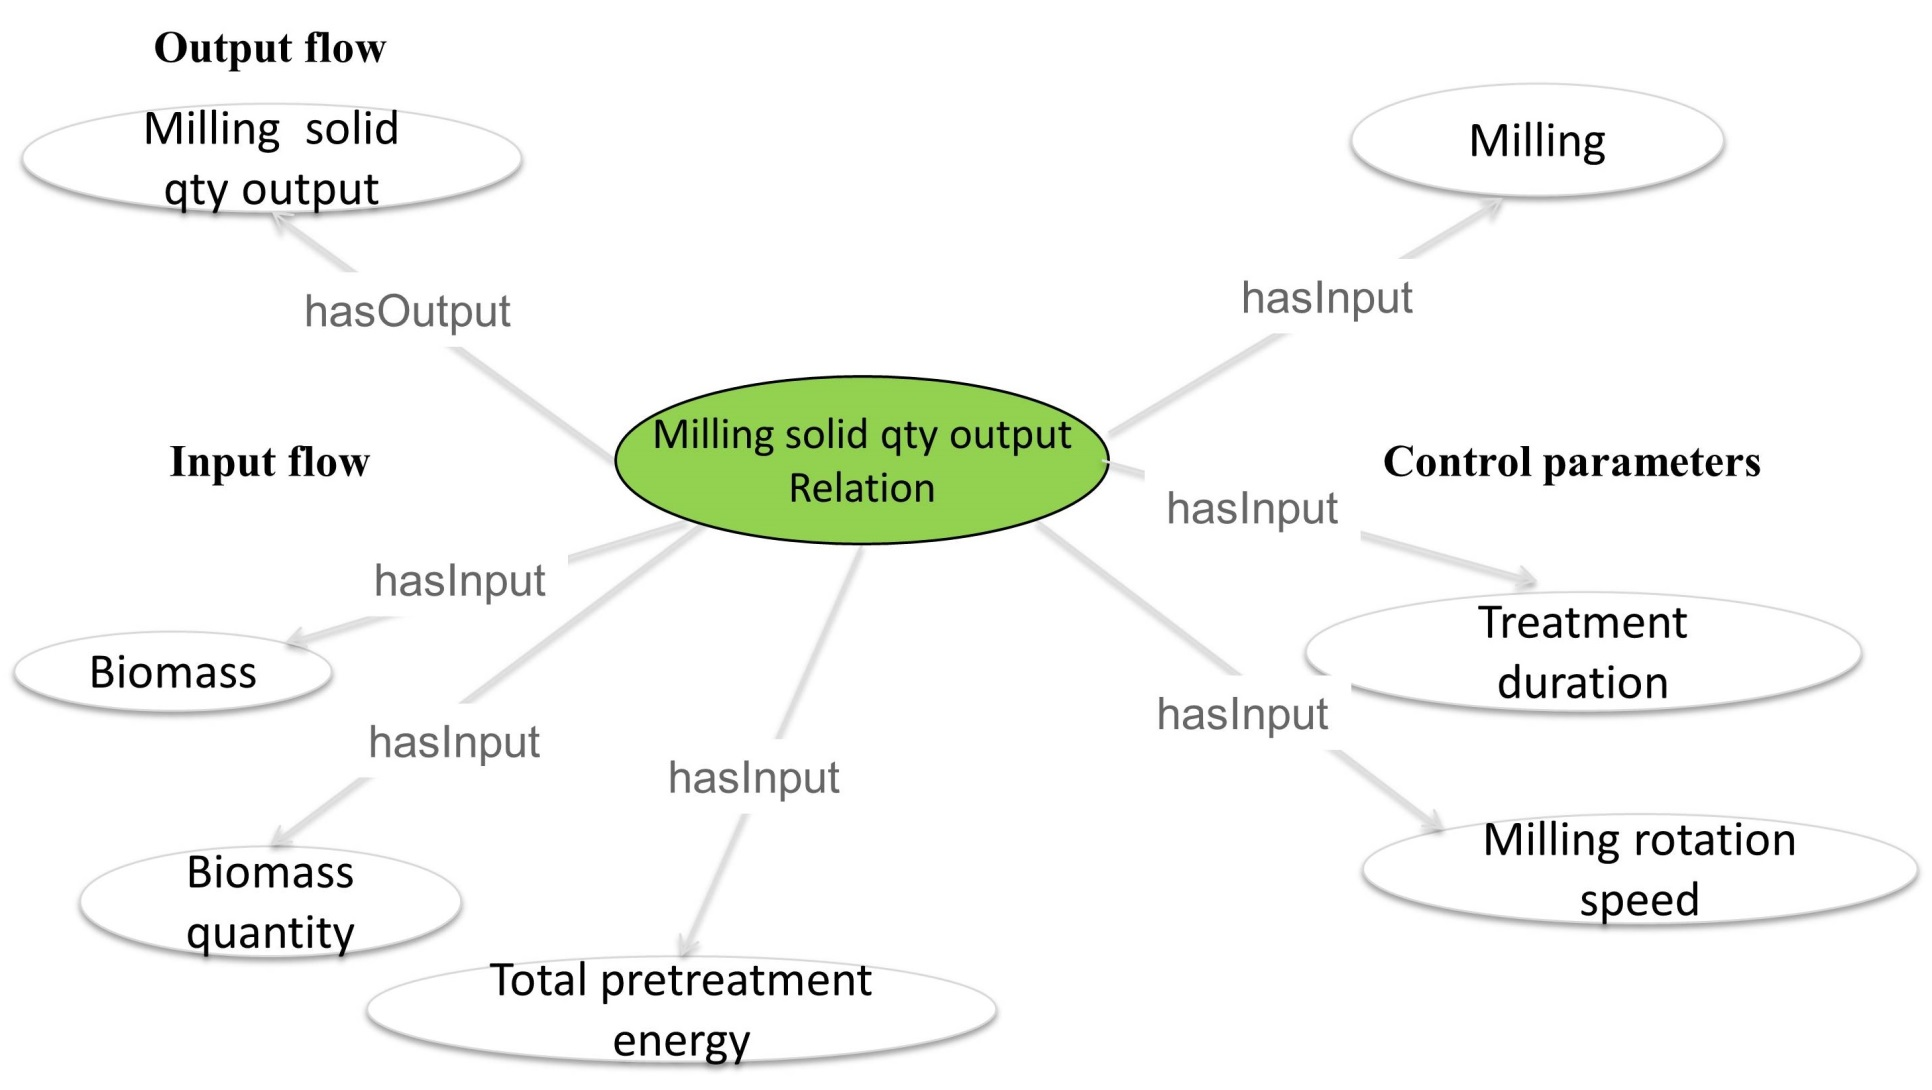
\includegraphics[width=10cm]{relation.jpg}
  \end{center}
\end{frame}

\begin{frame}
  \frametitle{\atweb ontology}

  \begin{center}
    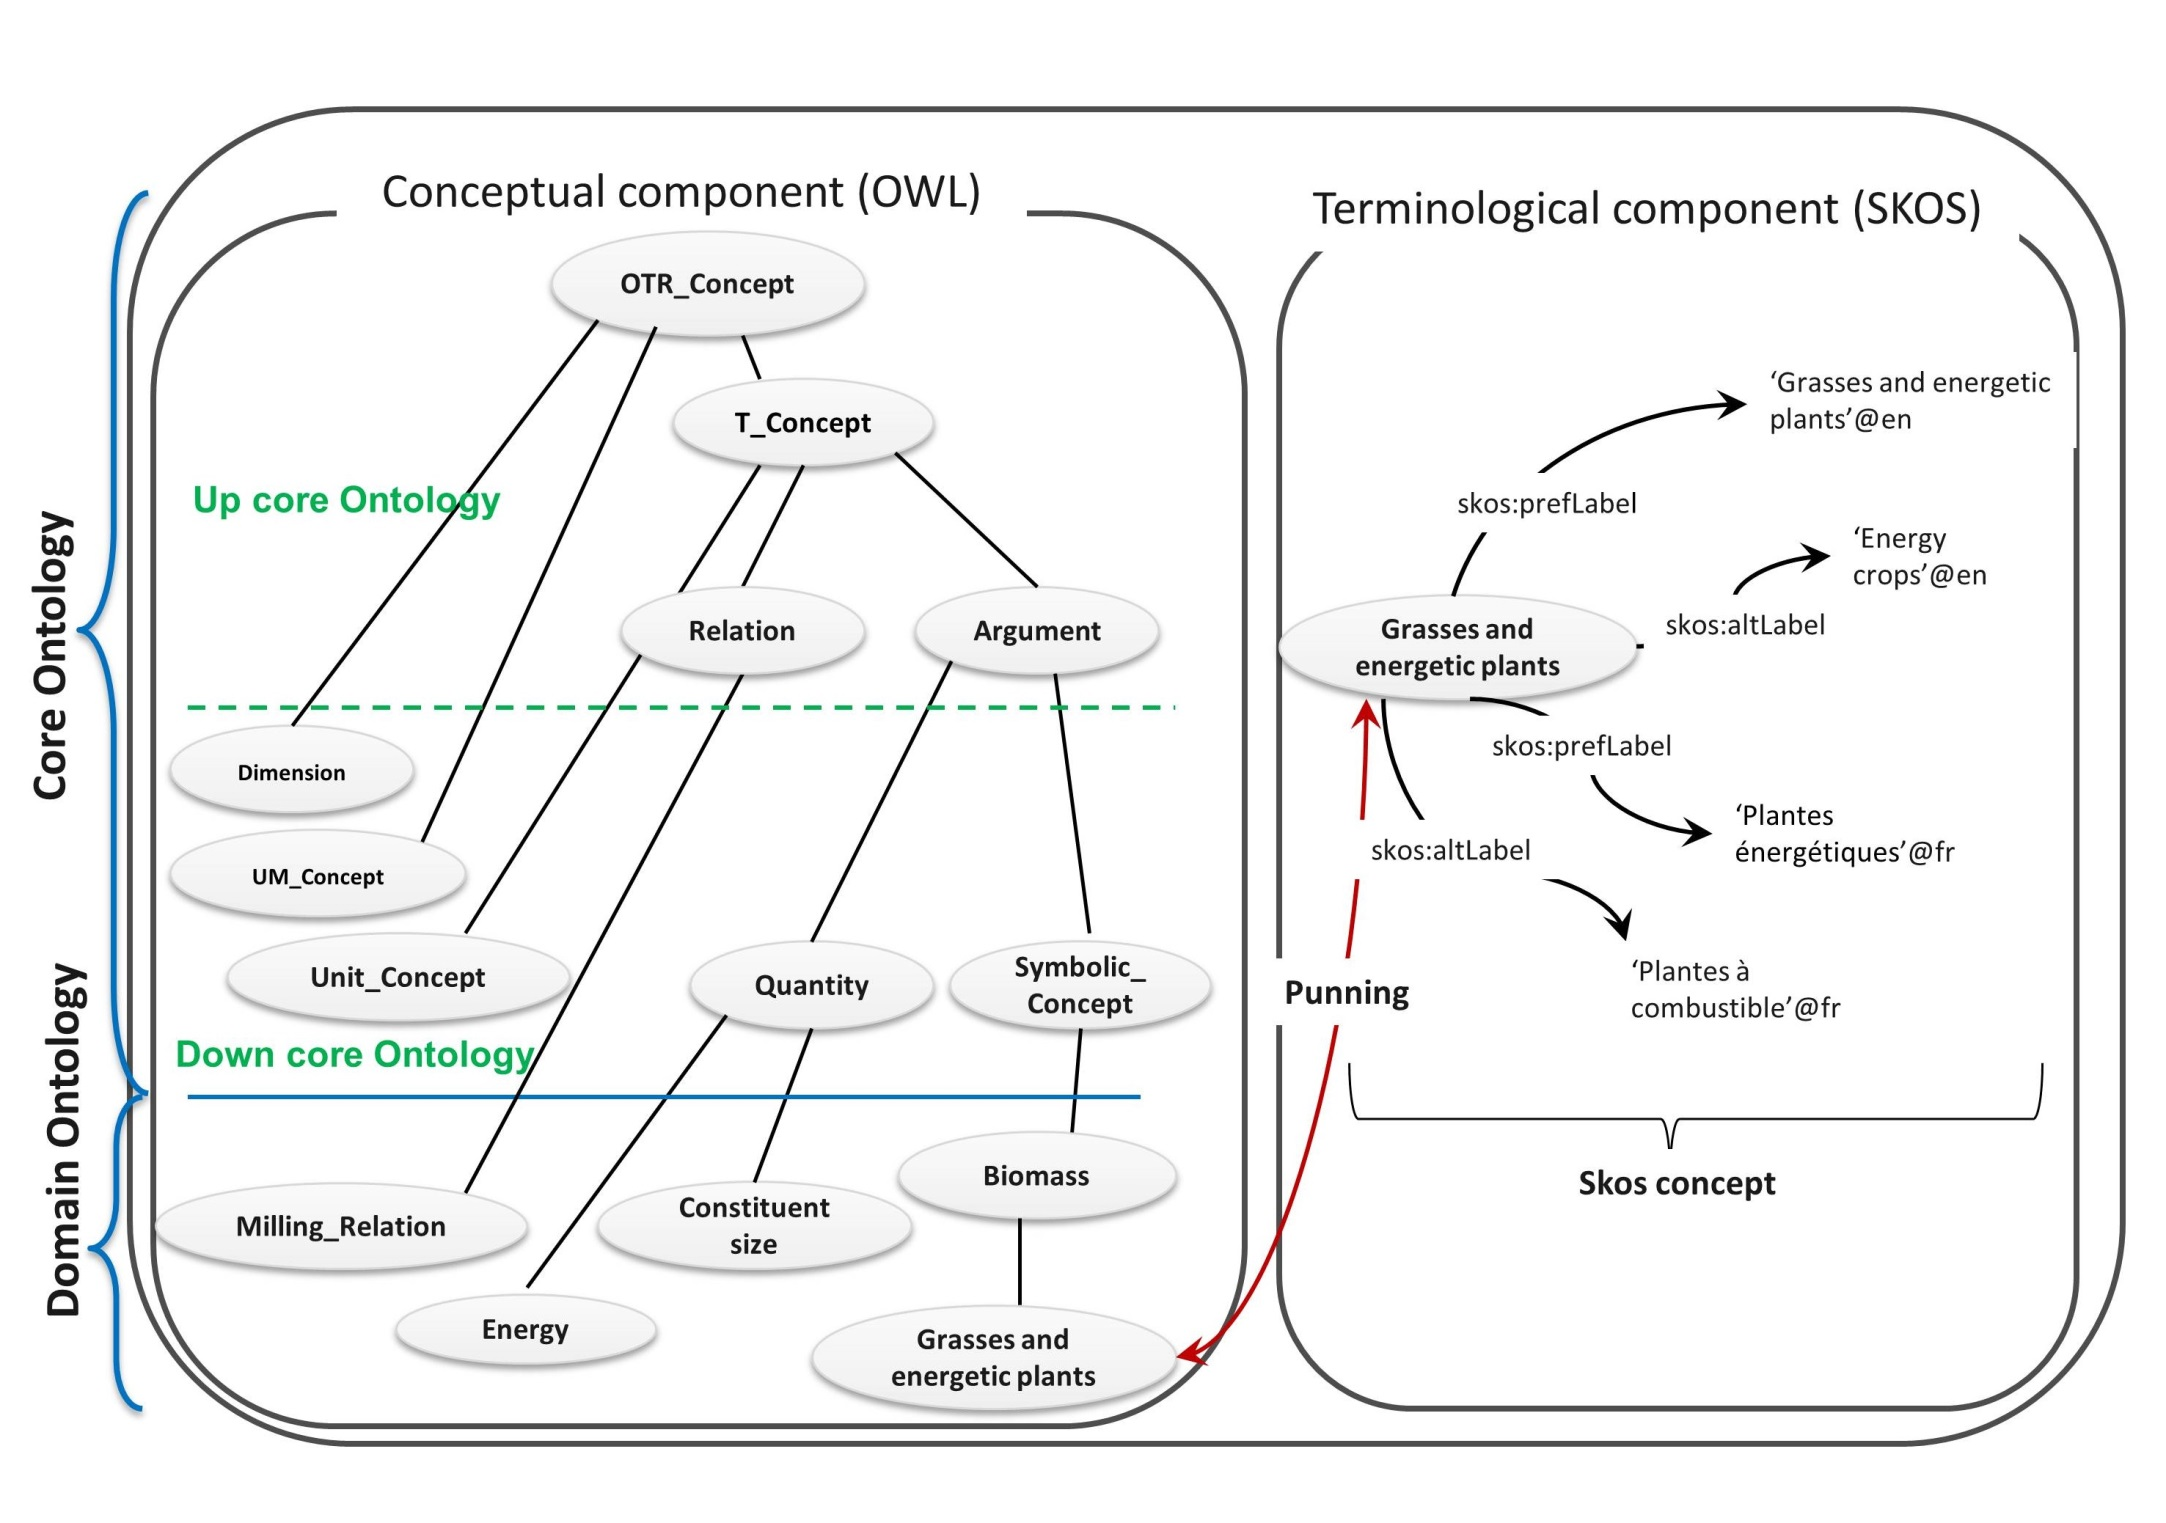
\includegraphics[width=10cm]{ontology.jpg}
  \end{center}
\end{frame}

\begin{frame}
  \frametitle{Annotated tables}
  \framesubtitle{Screenshot}

  \begin{center}
    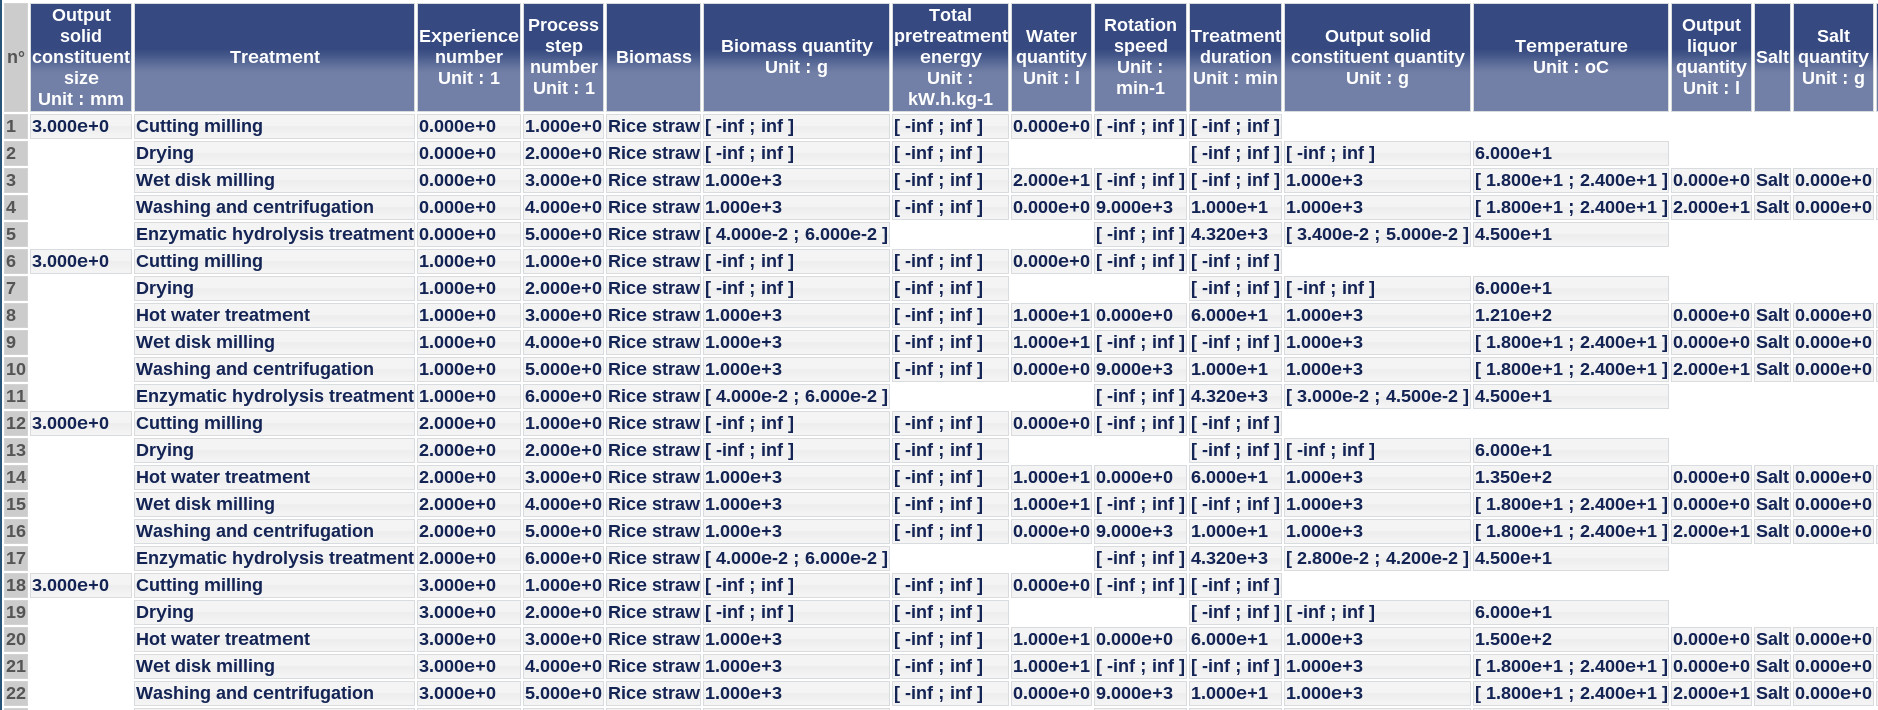
\includegraphics[width=11cm]{atweb-screenshot-table.jpg}
  \end{center}
\end{frame}

\begin{frame}
  \frametitle{Guidelines}

  \framesubtitle{Screenshot}

  \begin{center}
    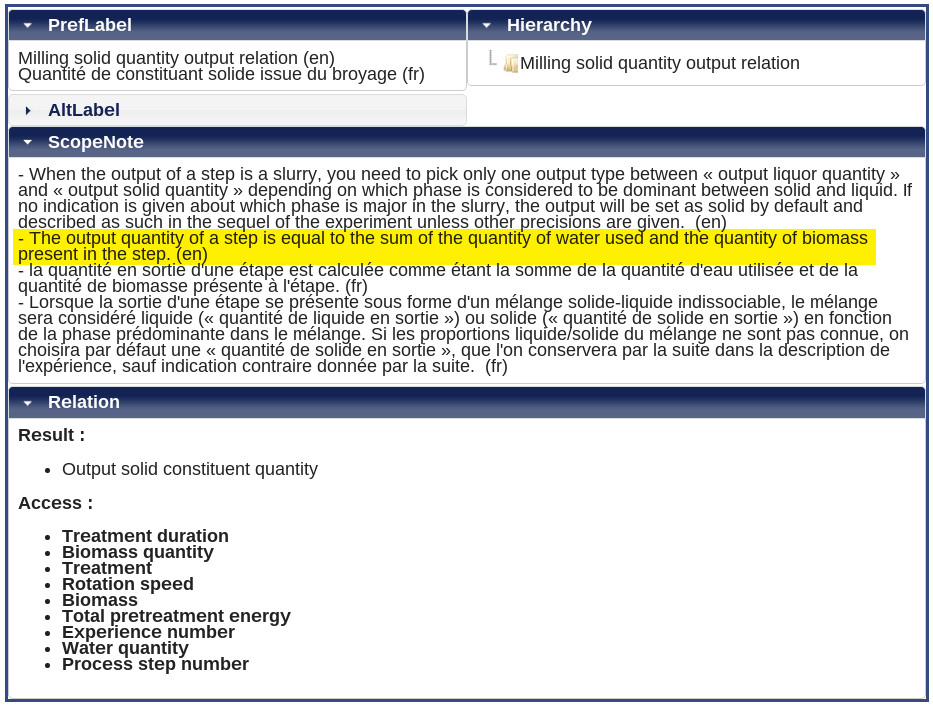
\includegraphics[width=10cm]{atweb-screenshot-guideline.jpg}
  \end{center}
\end{frame}

\begin{frame}
  \frametitle{Example guideline}
  \framesubtitle{Guideline}

  \textit{``The output quantity of a step is equal to the sum of the quantity
  of water used and the quantity of biomass present in the step.''}

  \pause

  $$output = waterInput + biomassInput$$
\end{frame}

\begin{frame}
  \frametitle{Example guideline}
  \framesubtitle{An annotated row that doesn't fulfill the guideline}

  \begin{center}
    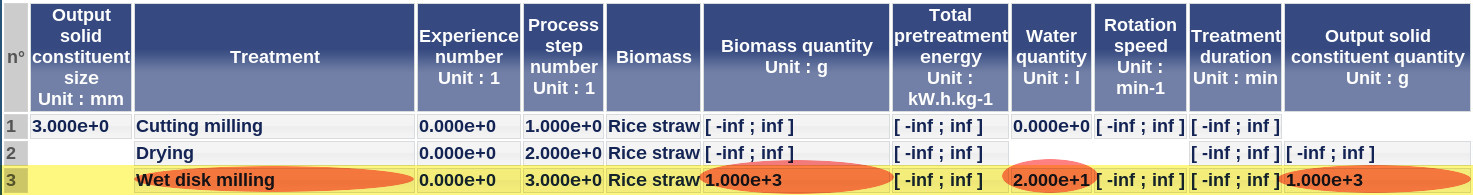
\includegraphics[width=11cm]{atweb-screenshot-row-with-relation.jpg}
  \end{center}

  \pause

  $$output = waterInput + biomassInput$$

  \pause

  {
    \color{red}
    $$1000 = 20 + 1000$$
  }
\end{frame}

%%%%%%%%%%%%%%%%%%%%%%%%%%%%%%%%%%%%%%%%%%%%%%%%%%%%%%%%%%%%%%%%%%%%%%%%%%%%%%%%
% Part II: RDF data validation: survey of the state of the art                 %
%%%%%%%%%%%%%%%%%%%%%%%%%%%%%%%%%%%%%%%%%%%%%%%%%%%%%%%%%%%%%%%%%%%%%%%%%%%%%%%%

\begin{frame}
  \partslide{Part II}{RDF data validation: survey of the state of the art}
\end{frame}

\begin{frame}
  \frametitle{Shape Expressions}

  Pending.
\end{frame}

\begin{frame}
  \frametitle{SHACL}

  Pending.
\end{frame}

\begin{frame}
  \frametitle{Plain SPARQL}

  Pending.
\end{frame}

%%%%%%%%%%%%%%%%%%%%%%%%%%%%%%%%%%%%%%%%%%%%%%%%%%%%%%%%%%%%%%%%%%%%%%%%%%%%%%%%
% Part III: Implementation                                                     %
%%%%%%%%%%%%%%%%%%%%%%%%%%%%%%%%%%%%%%%%%%%%%%%%%%%%%%%%%%%%%%%%%%%%%%%%%%%%%%%%

\begin{frame}
  \partslide{Part III}{Implementation}
\end{frame}

\begin{frame}
  \frametitle{Examples of real constraints}

  Pending.
\end{frame}

\begin{frame}
  \begin{center}
    \Huge{Demo}
  \end{center}
\end{frame}

%%%%%%%%%%%%%%%%%%%%%%%%%%%%%%%%%%%%%%%%%%%%%%%%%%%%%%%%%%%%%%%%%%%%%%%%%%%%%%%%
% Part IV: Conclusions                                                         %
%%%%%%%%%%%%%%%%%%%%%%%%%%%%%%%%%%%%%%%%%%%%%%%%%%%%%%%%%%%%%%%%%%%%%%%%%%%%%%%%

\begin{frame}
  \partslide{Part IV}{Conclusions}
\end{frame}

\begin{frame}
  \frametitle{Conclusions}

  Pending.
\end{frame}

\begin{frame}
  \frametitle{Future work}

  Pending.
\end{frame}

\begin{frame}
  \begin{center}
    \Huge{Thanks!}
  \end{center}
\end{frame}

% \begin{frame}
%   \frametitle{Motivation}
%   \framesubtitle{Problem statement}
%
%   \pause
%
%   \begin{itemize}
%     \item We're trying to answer questions that require consulting
%       heterogeneous data sources.
%
%     \pause
%
%     \begin{itemize}
%       \item Literature with inconsistent, semi-structured data.
%
%       \pause
%
%       \item No standard naming convention.
%
%       \pause
%
%       \item No information about the reliability of the data sources.
%
%       \pause
%
%       \item Each data source has its specific browsing/querying mechanism (no
%         common interface.)
%     \end{itemize}
%   \end{itemize}
% \end{frame}
%
% \begin{frame}
%   \frametitle{Motivation}
%   \framesubtitle{Sample problem domain: \textbf{biorefinery}}
%
%   \begin{itemize}
%     \item Ligno-cellulosic biomass pre-treatment before enzymatic hydrolysis is
%       an essential step to obtain good yields.
%
%     \pause
%
%     \item Several pre-treatment principles available, but \textbf{no clear
%       criteria on how to choose the best one} taking into account environmental
%       sustainability for a given biomass and biorefinery product (e.g.
%       glucose.)
%   \end{itemize}
% \end{frame}
%
% \begin{frame}
%   \frametitle{Proposed solution}
%
%   \begin{itemize}
%     \item Represent scientific knowledge with ontologies using recommended
%       standardized tools and languages for such purposes (semantic web
%       technologies, RDF(S), OWL, etc.)
%
%     \pause
%
%     \item Develop an ontology and data management web application (e.g. the
%       \textbf{@Web platform}) that makes it easy for scientists to introduce
%       data from scientific publications into an ontology, execute queries
%       against an ontology, etc.
%
%     \pause
%
%     \item Create integrity constraints to automatically detect inconsistencies
%       and errors in scientific publications and to automatically classify
%       publications according to their topics.
%
%     \pause
%
%     \begin{itemize}
%       \item \textit{The focus of my internship!}
%     \end{itemize}
%
%   \end{itemize}
% \end{frame}
%
% \begin{frame}
%   \frametitle{An example of a termino-ontological resource}
%   \framesubtitle{Taken from the biorefinery application}
%
%   \begin{center}
%     \includegraphics[width=10cm]{termino-ontological-resource.jpg}
%   \end{center}
% \end{frame}
%
% \begin{frame}
%   \frametitle{Design goals for the core ontology}
%
%   \begin{itemize}
%     \item \textbf{Simple} so as to make the annotator's task easier.
%
%     \pause
%
%     \item \textbf{Generic} enough so that the approach can be applied to
%       different, unrelated domains.
%
%     \pause
%
%     \begin{itemize}
%       \item Proven in the domains of biorefinery and packaging selection.
%     \end{itemize}
%   \end{itemize}
% \end{frame}
%
% \begin{frame}
%   \frametitle{A sample relation}
%   \framesubtitle{Also from the biorefinery domain}
%
%   \begin{center}
%     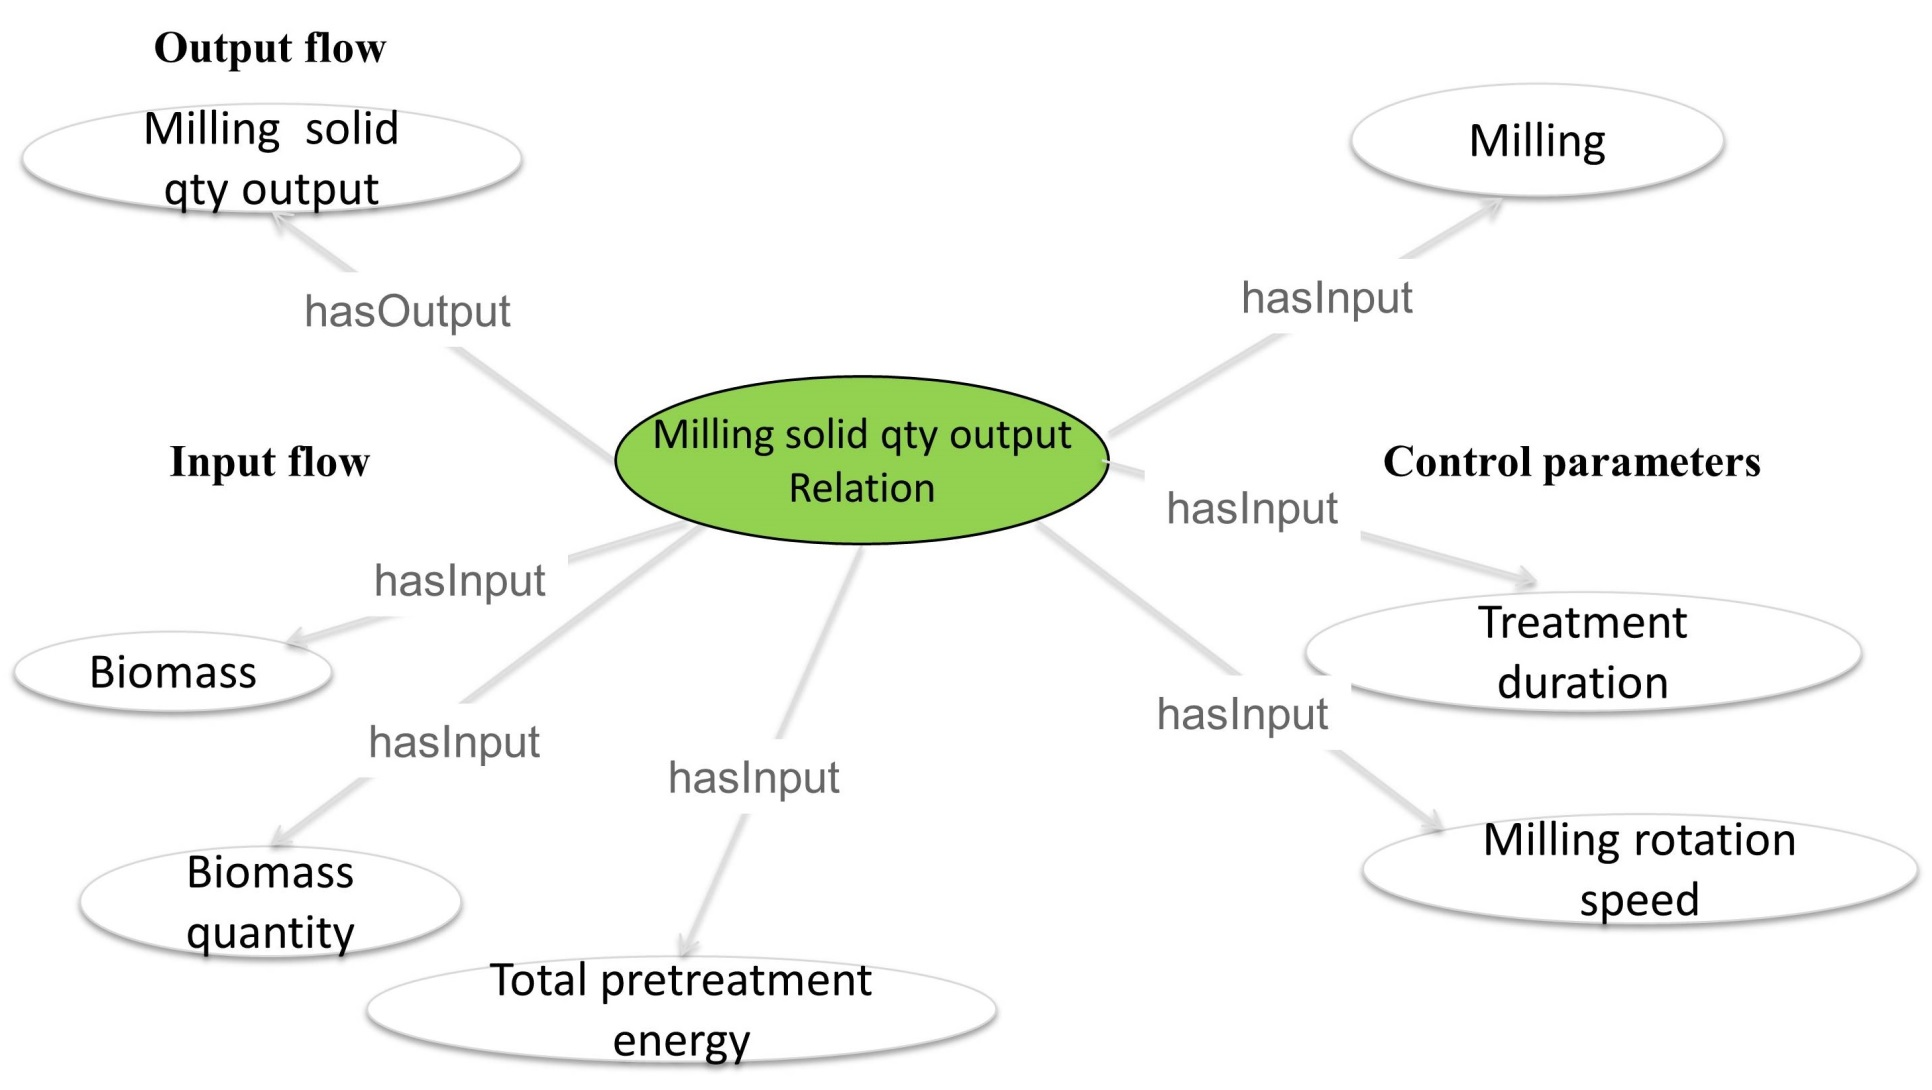
\includegraphics[width=10cm]{relation.jpg}
%   \end{center}
% \end{frame}
%
% \begin{frame}
%   \frametitle{The \textbf{@Web} platform}
%   \framesubtitle{Exploring an ontology}
%
%   \begin{center}
%     \includegraphics[width=8cm]{atweb-ontology.jpg}
%   \end{center}
% \end{frame}
%
% \begin{frame}
%   \frametitle{The \textbf{@Web} platform}
%   \framesubtitle{Browsing documents}
%
%   \begin{center}
%     \includegraphics[width=10cm]{atweb-document.jpg}
%   \end{center}
% \end{frame}
%
% \begin{frame}
%   \frametitle{The \textbf{@Web} platform}
%   \framesubtitle{Querying an ontology: defining the search scope}
%
%   \begin{center}
%     \includegraphics[width=10cm]{atweb-query-1.jpg}
%   \end{center}
% \end{frame}
%
% \begin{frame}
%   \frametitle{The \textbf{@Web} platform}
%   \framesubtitle{Querying an ontology: search parameters}
%
%   \begin{center}
%     \includegraphics[width=10cm]{atweb-query-2.jpg}
%   \end{center}
% \end{frame}
%
% \begin{frame}
%   \frametitle{The \textbf{@Web} platform}
%   \framesubtitle{Querying an ontology: executing a query}
%
%   \begin{center}
%     \includegraphics[width=10cm]{atweb-query-3.jpg}
%   \end{center}
% \end{frame}
%
% \begin{frame}
%   \frametitle{The \textbf{@Web} platform}
%   \framesubtitle{Querying an ontology: results}
%
%   \begin{center}
%     \includegraphics[width=10cm]{atweb-query-4.jpg}
%   \end{center}
% \end{frame}
%
% \begin{frame}
%   \frametitle{The annotator's task}
%
%   \begin{itemize}
%     \item Given a scientific publication and a desired ontology, capture data
%       from the publication using the appropriate concepts in the ontology.
%
%     \pause
%
%     \item Create and update concepts in the ontology as they're discovered
%       during the annotation process (i.e. in an iterative fashion.)
%
%     \pause
%
%     \item Write and edit \textbf{guidelines} associated to each concept
%       explaining when and how a concept should be used.
%   \end{itemize}
% \end{frame}
%
% \begin{frame}
%   \frametitle{An example of data captured from a scientific publication}
%
%   \begin{center}
%     \includegraphics[width=11cm]{table.jpg}
%   \end{center}
% \end{frame}
%
% \begin{frame}
%   \frametitle{A sample guideline}
%
%   \begin{center}
%     \includegraphics[width=10cm]{guideline.jpg}
%   \end{center}
% \end{frame}
%
% \begin{frame}
%   \frametitle{Some sample guidelines that can be easily translated into SPARQL
%   constraints}
%   \framesubtitle{Integrity constraints}
%
%   \begin{itemize}
%     \item \textit{``The output quantity of a step is equal to the sum of the
%       quantity of water used and the quantity of biomass present in the
%     step.''}
%
%     \pause
%
%     \item \textit{``The second milling step must give an “Output solid
%       constituent size” smaller than 0,5-1 mm.''}
%   \end{itemize}
% \end{frame}
%
% \begin{frame}
%   \frametitle{Some sample guidelines that can be easily translated into SPARQL
%   constraints}
%   \framesubtitle{Classification constraints}
%
%   \begin{itemize}
%     \item \textit{``Topic Bioref-PM-PC-UFM-PS : included experiments are
%       composed of a pre-milling step, followed by a physico-chemical treatment,
%     then by an ultrafine milling step (ball milling, wet disk milling, etc.), a
%   press and separation step (washing and filtration), and finally the enzymatic
% hydrolysis step. This topic requires a press and separation step because there
% are a lot of effluents in the physico-chemical step or because the milling is
% made with effluent. The second milling step must give an “Output solid
% constituent size” smaller than 0,5-1 mm. (en)''}
%   \end{itemize}
% \end{frame}
%
% \begin{frame}
%   \frametitle{Examples of guidelines that \textbf{cannot} be easily
%   translated into SPARQL constraints}
%
%   \begin{itemize}
%     \item \textit{``In all treatments, when the authors indicate ``overnight'',
%       we considered a duration treatment between 10 and 15 hours''}
%
%     \pause
%
%     \item \textit{``Furthermore, we consider that the glucose rate equals to
%       glucan rate divided by 0.9.''}
%   \end{itemize}
% \end{frame}
%
% \begin{frame}
%   \frametitle{Statistics}
%   \framesubtitle{A promising approach}
%
%   In the biorefinery ontology alone we have:
%
%   \begin{itemize}
%     \item 11 occurrences of the phrase \textit{``equal to''}
%     \item 5 occurrences of the phrase \textit{``equals to''}
%     \item 11 occurrences of the phrase \textit{``sum of''}
%     \item 3 occurrences of the phrase \textit{``divided by''}
%     \item 2 occurrences of the phrase \textit{``multiplied by''}
%   \end{itemize}
%
%   spread across guidelines associated with 30 relation concepts.
%
%   \vspace{1em}
%
%   \textbf{At least 10 of them can be easily translated into SPARQL constraints.}
% \end{frame}

\end{document}
